Kaon decays are powerful probes of new physics in the quark sector. The sensitivity of kaon observables to new physics in general surpasses that of $B$-meson decays, because of the stronger flavour (CKM and GIM) suppression factors of the SM contributions.  
Current experimental sensitivity 
already probes new physics scales 
up to $\sim 10^5$~TeV, as can be seen from Fig.~\ref{fig:NPscales} (in light green). 


\textbf{${K \to \pi \bar \nu \nu}$ decays}   are at present the driving goal of kaon physics. Their potential is due to the excellent theoretical precision, 
and to the possibility of disentangling different new physics models.
The SM predictions are BR($K^+ \to \pi^+ \bar \nu \nu$)$=(9.31 \pm 0.76)\times 10^{-11}$ and 
BR($K_L \to \pi^0 \bar \nu \nu$)$=(3.74 \pm 0.72)\times 10^{-11}$~\cite{Buras:2015qea,SozziESPP19}. 
An experiment aiming at the 10\% measurement for the $K^+$ decay rate is underway, and a discovery experiment for $K_L$ decay is running. 
In addition, several $K_L$-dedicated experiments aiming at the $15-20\%$ sensitivity are under proposal, and ultimate experiments  aiming  at the precision of a few $\%$ for both modes are being discussed.  

The {\bf charged kaon decay mode} 
has been measured at E787/E949~\cite{Artamonov:2009sz},
BR($K^+ \to \pi^+ \bar \nu \nu$)$=17.3^{+11.5}_{-10.5} \times 10^{-11}$. 
In the {\bf short-term}, NA62 is committed to deliver a measurement 
with $\mathcal{O}(10\%)$ precision 
prior to the Long Shutdown 3 (LS3). A feasibility study is also underway
to improve the precision of measurements 
at the higher beam intensities available after LS3~\cite{SozziESPP19,NA62:Lazzeroni}. 
For the {\bf neutral decay} mode, $K_L \to \pi^0 \bar \nu \nu$, the dedicated KOTO experiment at J-PARC 
has recently obtained the limit BR$(K_L \to \pi^0 \bar \nu \nu) < 3 \times 10^{-9}$ (90\% C.L.)~\cite{Ahn:2018mvc}. In the {\bf mid-/long-term}, both KOTO as well as the KLEVER project at CERN aim at significant progress. 
KOTO proposes to reach an $\mathcal{O}(100)$ SM event sensitivity 
by using the increase of the J-PARC Main Ring power to 100~kW and by upgrading the experiment~\cite{KOTO_prospects}. 
KLEVER~\cite{Ambrosino:2019qvz}, using the 400~GeV 
SPS proton beam, might start data taking during the LHC Run 4 (2026). The benchmark goal is to collect around 60 SM events in five years of data taking, assuming a
delivered intensity of $10^{19}$ pot/year. 
The joint prospects of KOTO and NA62 in the corresponding kaon decay
modes, as well as long term prospects including KLEVER and a second
phase KOTO-II (under discussion)~\cite{JPARC_EPPSU_input, KOTO_II},
are schematically depicted in Fig.~\ref{fig:Kpinunu.KOTO.NA62}. The  upcoming results expected  from NA62  and the evolution of the Japanese project will guide the future European steps in this research field.

Concerning the \textbf{$K_S$ decay modes}, the {\bf mid-term} prospects rely on the \HLLHC. 
The LHCb Upgrade II can approach the SM value 
BR($K_S \to \mu \mu$)$=5.2 \times 10^{-12}$~\cite{Cirigliano:2011ny}, and significantly improve the precision of the measurements done by NA48 (e.g.  $K_S \to \pi \mu \mu, \pi \pi e e$). The ultimate reach of LHCb Upgrade II could be $\mathcal{O}(10^{-15})$ for some $K_S$  decay modes~\cite{SozziESPP19}.  

Kaon decays further offer a good laboratory for \textbf{LFV, LNV} and lepton flavour universality violation (\textbf{LFUV}) searches, given
the high statistics, clean signatures and controlable backgrounds.
The $K^+$ and $K_L$ fluxes allow ``parasitic'' \textbf{charged LFV} decay searches below the $10^{-12}$ branching ratio level~\cite{SozziESPP19}.  For \textbf{LNV} decays, 
NA62 has already obtained the
bounds ${\rm BR}(K^+ \to \pi^- e^+e^+ (\mu^+\mu^+))<2.2(0.42)\times 10^{-10}$ 
at $90\%$ C.L.,  
from the 2017 data set~\cite{CortinaGil:2019dnd}.
In the {\bf short-term}, the full data collected for the latter modes will be about three times larger.  
{\bf LFUV} in kaon decays can be probed via the comparison of the helicity-suppressed widths, 
through the ratio 
$R_K^\ell = \Gamma (K^\pm \to e^\pm \nu)/\Gamma (K^\pm \to \mu^\pm\nu)$. 
In the {\bf short-term}, 
both TREK at J-PARC~\cite{JPARC_TREK} and NA62 are expected to reduce the current errors, 
 to 2.5~per mille and sub-per mille level, respectively~\cite{SozziESPP19,NA62:Lazzeroni}. 


New concepts to test {\bf discrete symmetries}
in kaon decays are being considered. 
As an example, TREK is  
exploring T violation in 
$K^+ \to \pi^0 \mu^+ \nu$. 
For the CP violation observables $\epsilon_K$ and $\epsilon^\prime/\epsilon$, no significant experimental developments are foreseen. 
On the theory side, however, progress in the computation of  the weak matrix elements and in the determination of the CKM angles will play a clear role. 
In particular, 
the first SM computation of $\epsilon^\prime/\epsilon$ with fully controlled uncertainties is expected in the short-term~\cite{Kelly:2019yxg}. 

The kaon sector also has a unique role in the determination of CKM elements, 
including new CKM unitarity tests through the emerging kaon unitarity triangle~\cite{Lehner:2015jga} (see Sect.~\ref{sec:CKM}). The sensitivity of related kaon observables to new physics  scales  is illustrated in Fig.~\ref{fig:NPscales} (present bounds from kaons and $B$ mesons in light green, LHCb Upgrade-II prospects in dark green).  

\begin{figure}
\begin{center}
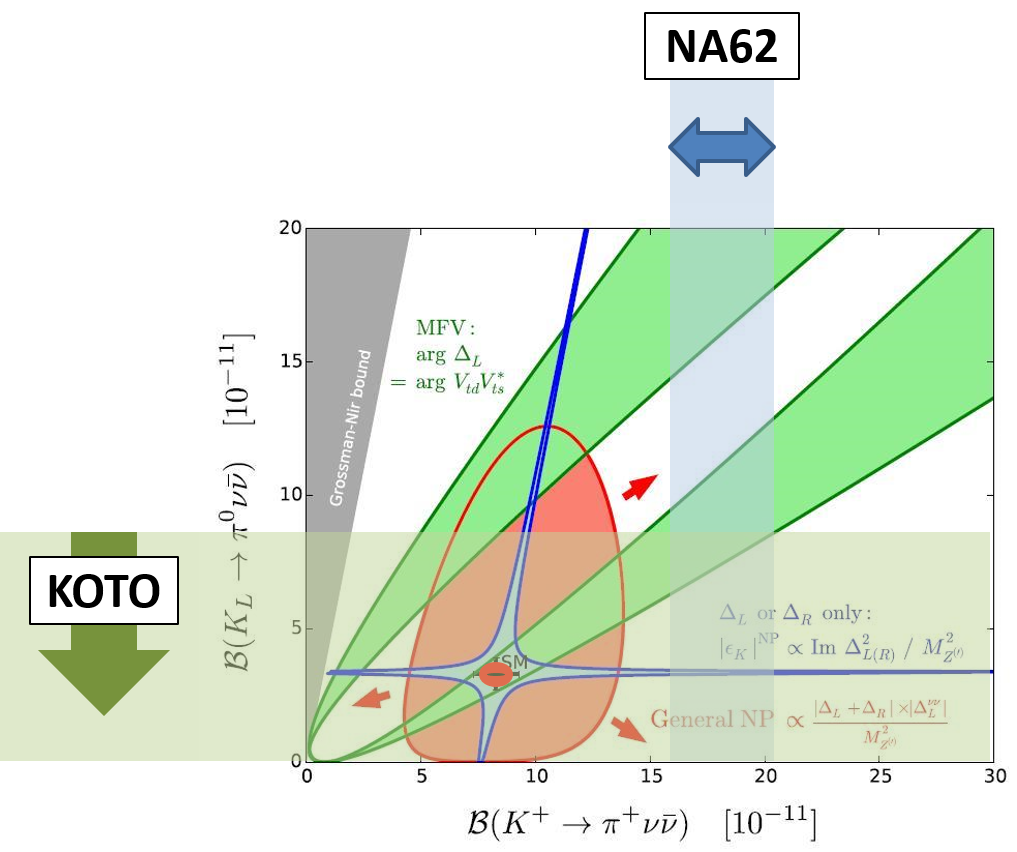
\includegraphics[width=0.45\textwidth]{\main/Flavour/figs/Figure1_kaon.png} 
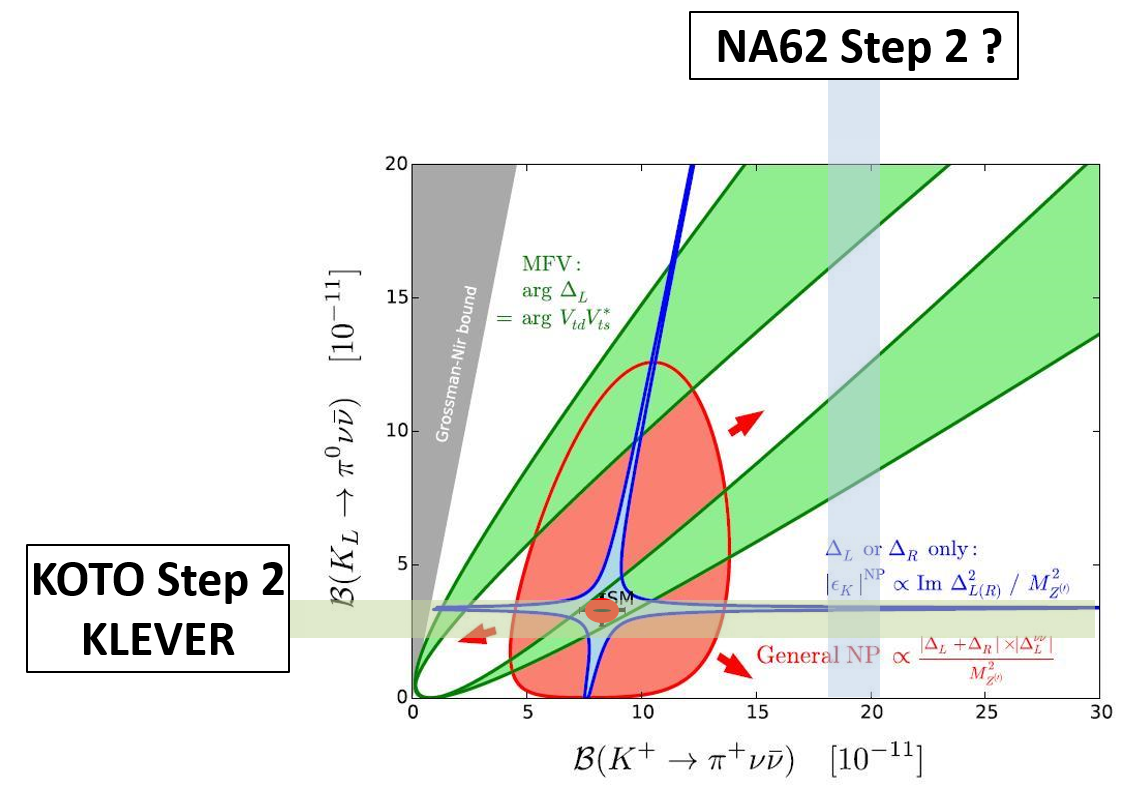
\includegraphics[width=0.49
\textwidth]{\main/Flavour/figs/Figure2_kaon.png} 
\end{center}
\caption{Educated guess for the future of the $K \to \pi \bar \nu \nu$
  decays (shaded vertical and horizontal regions): mid and long-term (respectively  
  left and right 
  panels)~\cite{SozziESPP19}. Original figure 
  from Ref.~\cite{Buras:2015yca}: the red region illustrates the lack of correlation for NP models with general left-handed and right-handed couplings; in green the correlation present in some MFV models; in blue the correlation induced by the constraint from $\epsilon_K$ if only left- or right-handed couplings are present.  
}
\label{fig:Kpinunu.KOTO.NA62}  
\end{figure}


Ultra-rare $K_L$ and $K^+$ decays are clearly the most-promising goal of the field.  Existing machines are fully adequate for the next step in kaon physics. However, ultimate discoveries require very high hadron intensities which could be provided in the {\bf long-term} by intense, high-duty-cycle extracted proton beams, such as from the J-PARC main ring, or from
the proton drivers required for a future hadron collider, with a beam power in the MW range.


